We use Modules for Experiments in Stellar Astrophysics
\citep[MESA][]{Paxton2011, Paxton2013, Paxton2015, Paxton2018, Paxton2019}.

https://www.overleaf.com/project/617b3cb8a0b9ee4a8f5db5fb
\section{1D calculations of stellar R0:Meridith}\label{sec:1D}
How is this done. math. any tricks related to extracting these things from MESA. averaging etc. cite previous work.

make plot of mass versus metallicity color coded by R0 at the RGB bump.


To make Adrian happy: run models and extract the fluid parameters at various time steps (onset of thermohaline, when thermohaline touches scz for the first time, all timesteps in between). How do the fluid parameters and change at these various timesteps. how do the ratios between different models depend on which timesteps you choose (hopefully not at all). Also run at different thermohaline proscriptions. Does that matter? Assuming it isn't grossly awful, proceed to the next step.

{\color{red} Evan describe the algorithm for going from mesa model to r value}.

\begin{figure*}
    \centering
    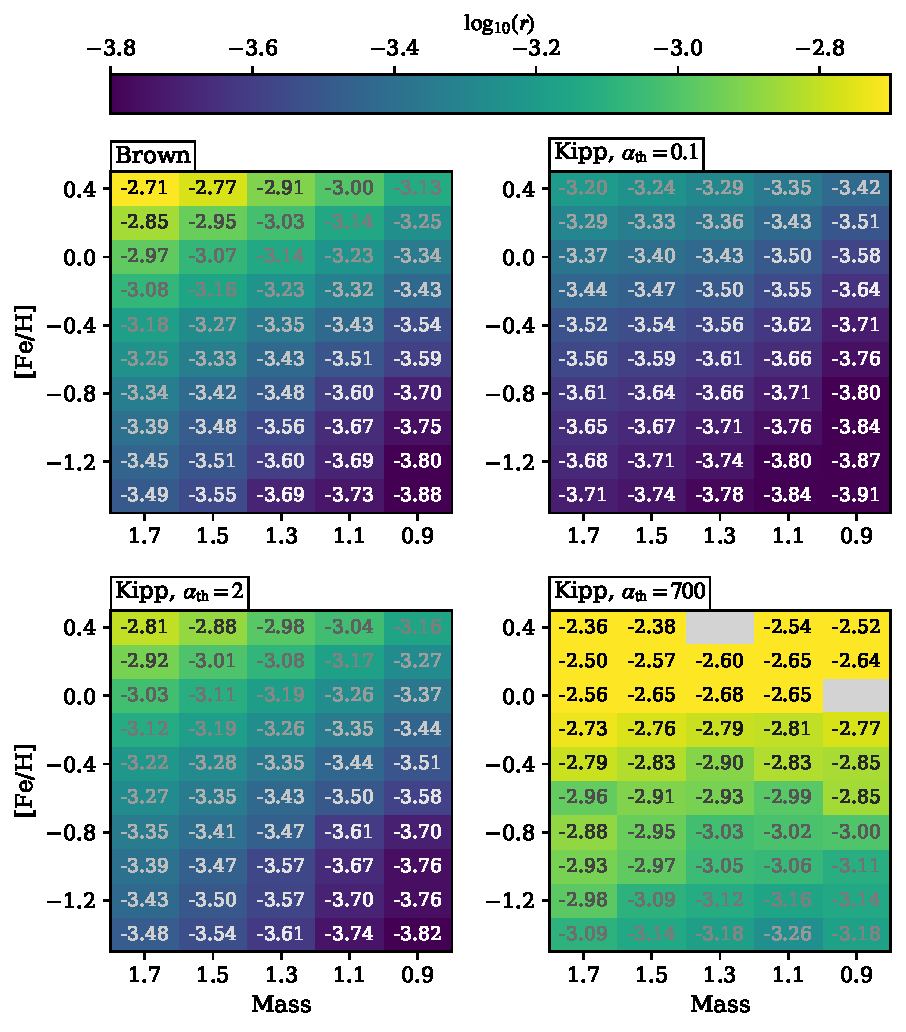
\includegraphics[width=\textwidth]{figures/mesa_spread/mesa_r_spread.pdf}
    \caption{This is a caption. {\color{red} Evan add a description of what model is used in each grid}}
    \label{fig:mesa_r_spread}
\end{figure*}